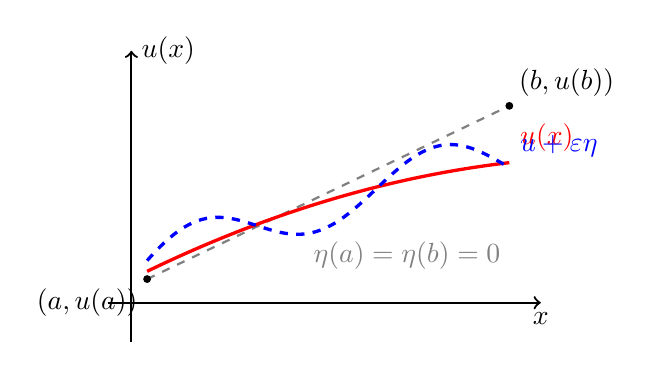
\begin{tikzpicture}[scale=1.0]
  % axes
  \draw[->, thick] (0,-0.5) -- (0,3.2) node[right] {$u(x)$};
  \draw[->, thick] (-0.3,0) -- (5.2,0) node[below] {$x$};

  % endpoints
  \coordinate (A) at (0.2, 0.3);
  \coordinate (B) at (4.8, 2.5);
  \draw[gray, dashed, thick] (A) -- (B);

  % nominal curve y = u(x)
  \draw[red, very thick, domain=0.2:4.8, samples=80]
    plot (\x, {0.3 + 0.5*\x - 0.04*\x*\x}) node[above right] {$u(x)$};

  % varied curve u + eps eta
  \draw[blue, very thick, dashed, domain=0.2:4.8, samples=80]
    plot (\x, {0.3 + 0.5*\x - 0.04*\x*\x + 0.35*sin(deg(2*\x))})
         node[above right] {$u+\varepsilon\eta$};

  % labels
  \filldraw (A) circle (1.2pt) node[below left] {$(a,u(a))$};
  \filldraw (B) circle (1.2pt) node[above right] {$(b,u(b))$};
  \node[gray] at (3.5, 0.6) {$\eta(a)=\eta(b)=0$};
\end{tikzpicture}